
\frame{
\frametitle{Gui: Klassendiagramm}
	\begin{center}
		\begin{figure}
			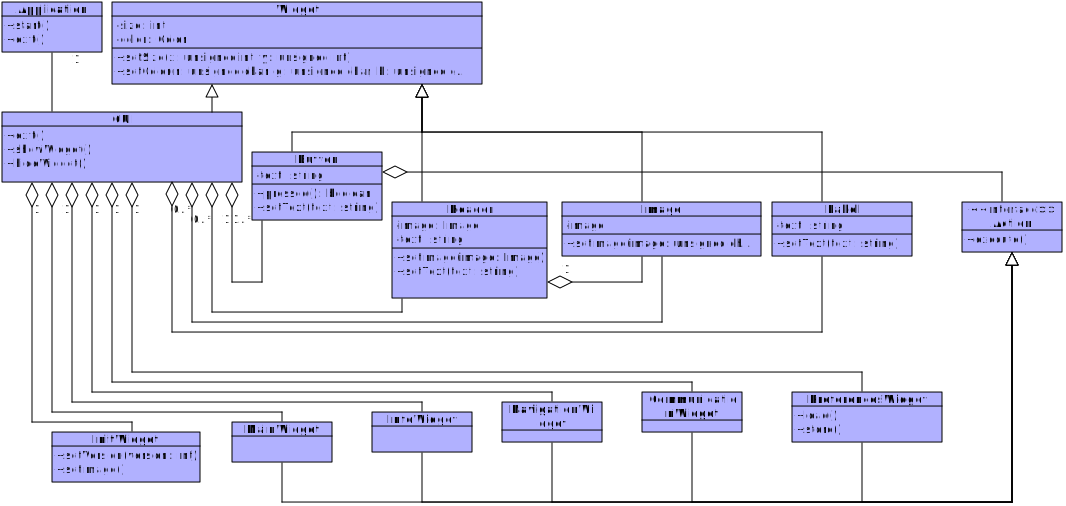
\includegraphics[width=1.0\textwidth]{../grafiken/GUI_Class.pdf}
			\caption{Klassendiagramm für Programmstruktur. }		
		\end{figure}
	\end{center}
}

\frame{
\frametitle{Menüwechsel}
	\begin{block}{Zustandsmaschine}
		\begin{itemize}
			\item \textbf{Menüpunkte} werden als \textbf{Zustand} gesehen
			\item zusätzliche Zustände für \textbf{Start und Beenden} der Application
			\item Zustände können wiederum Unter-Zustände besitzen
		\end{itemize}
		\begin{center}
			\begin{figure}
				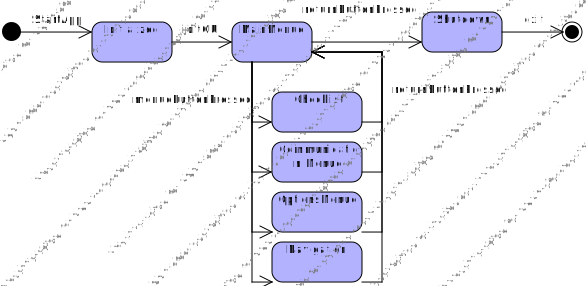
\includegraphics[width=0.55\textwidth]{../grafiken/MenueStates.pdf}
				\caption{State Machine ausgelöst durch das Interface \textit{Action}}
			\end{figure}
		\end{center}
	\end{block}
}
